\documentclass[final,12pt]{colt2018}

\usepackage{algorithm}
\usepackage{algorithmic}
\renewcommand{\algorithmicrequire}{\textbf{Input:}}
\renewcommand{\algorithmicensure}{\textbf{Output:}}

\usepackage{thmtools,thm-restate}

% For notes
\def\shownotes{0}  %set 1 to show author notes
\ifnum\shownotes=1
\newcommand{\authnote}[2]{{$\ll$\textsf{\footnotesize #1 notes: #2}$\gg$}}
\else
\newcommand{\authnote}[2]{}
\fi
\newcommand{\yingyu}[1]{{\color{blue}\authnote{Yingyu}{{#1}}}}
\newcommand{\yuanzhi}[1]{{\color{red}\authnote{Yuanzhi}{{#1}}}}


\usepackage{multirow}


\newcommand{\var}{\textsf{Var}}
\newcommand{\veps}{\varepsilon}
\newcommand{\bI}{\bold{I}}
\newcommand{\bM}{\bold{M}}
\newcommand{\bA}{\bold{A}}
\newcommand{\bX}{\bold{X}}
\newcommand{\bY}{\bold{Y}}
\newcommand{\bV}{\bold{V}}
\newcommand{\bU}{\bold{U}}
\newcommand{\bSigma}{\bold{\Sigma}}	
\newcommand{\E}{\mathbb{E}}
\DeclareMathOperator*{\argmin}{arg\,min}
\DeclareMathOperator*{\sign}{sign}




\title{Learning Mixtures of Linear Regressions with Nearly Optimal Complexity}
\usepackage{times}

\coltauthor{\Name{Yuanzhi Li} \Email{yuanzhil@cs.princeton.edu}\\
 \addr Princeton University, Computer Science Department
 \AND
 \Name{Yingyu Liang} \Email{yliang@cs.wisc.edu}\\
 \addr University of Wisconsin-Madison, Computer Sciences Department
 }

\begin{document}

\maketitle


\begin{abstract}
Mixtures of Linear Regressions (MLR) is an important mixture model with many applications. In this model, each observation is generated from one of the several unknown linear regression components, where the identity of the generated component is also unknown. Previous works either assume strong assumptions on the data distribution or have high complexity. This paper proposes a fixed parameter tractable algorithm for the problem under general conditions, which achieves global convergence and the sample complexity scales nearly linearly in the dimension. In particular, different from previous works that require the data to be from the standard Gaussian, the algorithm allows the data from Gaussians with different covariances. When the conditional number of the covariances and the number of components are fixed, the algorithm has nearly optimal sample complexity $N = \tilde{O}(d)$ as well as nearly optimal computational complexity $\tilde{O}(Nd)$, where $d$ is the dimension of the data space. To the best of our knowledge, this approach provides the first such recovery guarantee for this general setting.
\end{abstract}


% !TeX root = main.tex
\section{Introduction}
\label{sec:intro}
Generative models are often trained in an unsupervised fashion, fitting a model $q$ to a set of observed data $x_P \subseteq X$ drawn iid from some true distribution $p$ on $x\in X$. Now, of course $p$ may not exactly belong to family $Q$ of probability distributions being fit, whether $Q$ consists of Gaussians mixture models, Markov models, or even neural networks of bounded size. We first discuss the limitations of generative modeling without feedback, and then discuss our model and results.

%\subsection{Limitations of Generative Modeling from Positive Examples Alone}
Consider fitting a generative model on a text corpus consisting partly of poetry written by four-year-olds and partly of mathematical publications from the {\em Annals of Mathematics}. Suppose that learning to generate a poem that looks like it was written by a child was easier than learning to generate a novel mathematical article with a correct, nontrivial statement. If the generative model pays a high price for generating unrealistic examples, then it may be better off learning to generate children's poetry than mathematical publications. However, without negative feedback, it may be difficult for a neural network or any other model to know that the mathematical articles it is generating are stylistically similar to the mathematical publications but do not contain valid proofs.\footnote{This is excluding clearly fake articles published without proper review in lower-tier venues \citep{LabbeL13}.} 

As a simpler example, the classic Markovian ``trigram model'' of natural language assigns each word a fixed probability conditioned only on the previous two words. Prior to recent advances in deep learning, for decades the trigram model and its variant were the workhorses of language modeling, assigning much greater likelihood to natural language corpora than numerous linguistically motivated grammars and other attempts \citep{Rosenfeld00}. However, text sampled from a trigram is typically nonsensical, e.g., the following text was randomly generated from a trigram model fit on a corpus of text from the Wall Street Journal \citep{JurafskyM09}:
\begin{quote}
They also point to ninety nine point six billion dollars from two hundred
four oh six three percent of the rates of interest stores as Mexico and
gram Brazil on market conditions. 
\end{quote}

In some applications, like text compression using a language model \citep{WittenNC87}, maximizing likelihood is equivalent to optimizing compression. However, in many  applications involving generation, such nonsense is costly and unacceptable. Now, of course it is possible to always generate valid data by returning random training examples, but this is simply overfitting and not learning. Alternatively, one could incorporate human-in-the-loop feedback such as through crowdsourcing, into the generative model to determine what is a valid, plausible sentence.

In some domains, validity could be determined automatically. Consider a Markovian model of a well-defined concept such as mathematical formulas that compile in \LaTeX{}. Now, consider a $n$-gram Markovian character model which the probability of each subsequent character is determined by the previous $n$ characters. For instance, the expression \$\{2+\{x-y\}\$ is invalid in \LaTeX{} due to mismatched braces. For this problem, a \LaTeX{} compiler may serve as a validity oracle. Various $n$-gram models can be fit which only generate valid formulas. To address mismatched braces, for example, one such model would ensure that it always closed braces within $n$ characters of opening, and had no nested braces. While an $n$-gram model will not perfectly model the true distribution over valid \LaTeX{} formulas, for certain generative purposes one may prefer an $n$-gram model that generates valid formulas over one that assigns greater likelihood to the training data but generates invalid formulas. 

Figure \ref{fig:rectangle} illustrates a simple case of learning a rectangle model for data which is not uniform over a rectangle. A maximum likelihood model would necessarily be the smallest rectangle containing all the data, but most examples generated from this distribution may be invalid. Instead a smaller rectangle, as illustrated in the figure, may be desired.

\begin{figure}[h]\label{fig:rectangle}
\centering
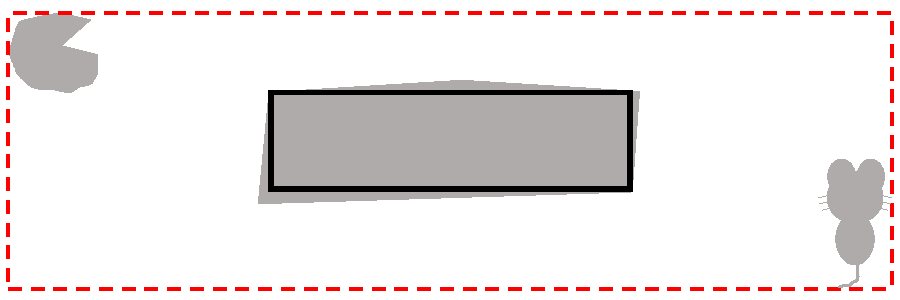
\includegraphics[width=3in]{fig.pdf}
\caption{Example where the underlying distribution $p$ is uniform over the (gray) valid regions. The solid rectangle maximizes our objective since it does not output nonsense (is supported only within the grey matter) and is closest to the $p$ (covers the maximum amount of grey matter). In contrast, the standard maximum likelihood (dashed red) rectangle must fully contain the observed samples, thus generating invalid points most of the time.  }
\end{figure}

Motivated by these observations, we evaluate a generative model $q$ on two axes. First is {\em coverage}, which is related to the probability assigned to future examples drawn from the true distribution $p$. Second is {\em validity}, defined as the probability that random examples generated from $q$ meet some validity requirement. Formally, we measure coverage in terms of a bounded {\em loss}:
$$\Loss(p,q)=\E_{x \sim p}[L(q_x)],$$
where $L:[0,1]\rightarrow [0,M]$ is a bounded decreasing function such as the capped log-loss $L(q_x)=\min(M, \log 1/q_x)$. % or $L(q_x)=\log 1/(q_x+\exp(-M))$. 
A bounded loss has the advantages of being efficiently estimable, and also it enables a model to assign 0 probability to one example (e.g., an outlier or error) if it greatly increases the likelihood of all other data. Validity is defined with respect to a set $V \subseteq X$, and $q(V)$ is the probability that a random example generated from $q$ lies within $V$. 

Clearly, there is a tradeoff between coverage and validity. We first focus on the case of (near) perfect validity. A Valid Generative Modeling (VGM) algorithm if it outputs, for a family of distributions $Q$ over $X$, if it outputs $\hat{q}$ with (nearly) perfect validity and whose loss is nearly as good as the loss of the best valid $q\in Q$. More precisely, $A$ is a VGM learner of $Q$ if for any nonempty valid subset $V \subseteq X$, any probability distribution $p$ over $V$, and any $\eps>0$, $A$ uses $n$ random samples from $p$ and makes $m$ membership oracle calls to $V$ and outputs a distribution $\hat{q}$ such that, $$\Loss(p, \hat{q}) \leq \min_{q \in Q: q(V)=1}\Loss(p,q) + \eps ~\text{ and }~\hat{q}(V)\geq 1-\eps.$$ 
We aim for our learner to be sample and query efficient, requiring that $n$ and $m$ are polynomial in $M, 1/\eps$ and a measure of complexity of our distribution class $Q$.
Furthermore, we would like our algorithms to be computationally efficient, with a runtime polynomial in the size of the data, namely the $n + m$ training examples. 
A more formal description of the problem is available in Section~\ref{sec:problem}.

$A$ is said to be {\em proper} if it always outputs $\hat{q}\in Q$ and {\em improper} otherwise.
In Section~\ref{sec:impossibility}, we first show that efficient proper learning for VGM is impossible. This is an information-theoretic result, meaning that even given infinite runtime and positive samples, one still cannot solve the VGM problem. Interestingly, this is different from binary classification, where it is possible to statistically learn from iid examples without a membership oracle.

Our first main positive result is an efficient (improper) learner for VGM. The algorithm relies on a subroutine that solves the following {\em Generative Modeling with Negatives} (GMN) problem: given sets $X_P, X_N \subset X$ of positive and negative examples, find the probability distribution $q \in Q$ which minimizes $\sum_{x \in X_P} L(q(x))$ subject to the constraint that $q(X_N)=0$. For simplicity, we present our algorithm for the case that the distribution family $Q$ is finite, giving sample and query complexity bounds that are logarithmic in terms of $|Q|$. However, as we show in Section~\ref{sec:infinite-families}, all of our results extend to infinite families $Q$. It follows that if one has a computationally efficient algorithm for the GMN problem for a distribution family $Q$, then our reduction gives a computationally efficient VGM learning algorithm for $Q$.

Our second positive result is an algorithm that minimizes $\Loss(p,q)$ subject to a relaxed validity constraint comparing against the optimal distribution that has validity $q(V)$ at least $1-\alpha$ for some $\alpha>0$. We show in Section~\ref{sec:partial-validity} that even in this more general setting, it is possible to obtain an algorithm that is statistically efficient but may not be computationally efficient. An important open question is whether there exists a computationally efficient algorithm for this problem when given access to an optimization oracle, as was the case for our algorithm for VGM.

\subsection{Related Work}
\cite{KearnsMRRSS94} showed how to learn distributions from positive examples in the realizable setting, i.e., where the true distribution is assumed to belong to the class being learned. In the same sense as their work is similar to PAC learning \citet{Valiant84} of distributions, our work is like agnostic learning \citet{KearnsSS94} in which no assumption on the true distribution is made. 

Generative Adversarial Networks (GANs)~\cite{GoodfellowPMXWOCB14} are an approach for generative modeling from positive examples alone, in which a generative model is trained against a discriminator that aims to distinguish real data from generated data. In some domains, GANs have been shown to outperform other methods at generating realistic-looking examples. Several shortcomings of GANs have been observed \citet{AroraRZ18}, and GANs are still subject to the theoretical limitations we argue are inherent to any model trained without a validity oracle. 

In supervised learning, there is a rich history of learning theory with various types of queries, including membership which are not unlike our (in)validity oracle. Under various assumptions, queries have been shown to facilitate the learning of complex classes such as finite automata \citet{Angluin88} and DNFs \citet{Jackson97}. See the survey of \cite{Angluin92} for further details.  Interestingly, \cite{Feldman09} has shown that for agnostic learning, i.e., without making assumptions on the generating distribution, the addition of membership queries does not enhance what is learnable beyond random examples alone. 
Supervised learning also has a large literature around active learning, showing how the ability to query examples reduces the sample complexity of many algorithms. See the survey of \cite{Hanneke14}. Note that the aim here is typically to save examples and not to expand what is learnable.
 
More sophisticated models, e.g., involving neural networks, can mitigate the invalidity problem as they often generate more realistic natural language and have even been demonstrated to generate \LaTeX{} that nearly compiles \citep{Karpathy15} or nearly valid Wikipedia markdown. However, longer strings generated are unlikely to be valid. For example, \cite{Karpathy15} shows generated markdown which includes:
\begin{quote}
==Access to ''rap===
The current history of the BGA has been [[Vatican Oriolean Diet]], British Armenian, published in 1893.  While actualistic such conditions such as the [[Style Mark Romanians]] are still nearly not the loss.
\end{quote}

Even ignoring the mismatched quotes and equal signs, note that this example has two so-called ``red links'' to two pages that do not exist. Without checking, it was not obvious to us whether or not Wikipedia had pages titled {\em Vatican Oriolean Diet} or {\em Style Mark Romanians}. In some applications, one may or may not want to disallow red links. In the case that they are considered valid, one may seek a full generative model of what might plausibly occur inside of brackets, as the neural network has learned in this case. If they are disallowed, a model might memorize links it has seen but not generate new ones. A validity oracle can help the learner identify what it should avoid generating.

 In practice, \cite{KusnerPH17} discuss how generative models from neural networks (in particular autoencoders) often generate invalid sequences. 
\cite{JanzWPKH18} learn the validity of examples output by a generative model using oracle feedback. 

\section{Related Work} \label{sec:related}


Mixtures of Linear Regressions is a popular mixture model (e.g.,~\citep{de1989mixtures,grun2007applications} and \citep{faria2010fitting}), also known as Hierarchical Mixture of Experts in~\citep{jordan1994hierarchical} in the machine learning community. 
It has many applications, such as trajectory clustering~\citep{gaffney1999trajectory} and phase retrieval~\citep{balakrishnan2017statistical}, and has as special cases some popular models, such as piecewise linear regression and locally linear regression.

Learning MLR in general is NP-hard~\citep{yi2014alternating}. Recent interests have been in providing various efficient algorithms for recovering the parameters in MLR under assumptions about the data generation model~\citep{chaganty2013spectral,chen2014convex,yi2014alternating,zhong2016mixed,klusowski2017estimating}. 
%These results assumes the data $x$ in different components are all from the standard Gaussians. 
They are either under restricted assumptions about the data (mixtures of two component or $x$ all from the standard Gaussian)~\citep{chen2014convex,yi2014alternating,balakrishnan2017statistical,klusowski2017estimating}, or have high sample or computational complexity~\citep{chaganty2013spectral,sedghi2016provable}. 

Some works study specific algorithms for the problem, such as  the Expectation Maximization (EM) algorithm~\citep{khalili2007variable,yi2014alternating,balakrishnan2017statistical,klusowski2017estimating}. It is known that without careful initialization EM is only guaranteed to have local convergence~\citep{klusowski2017estimating}. A grid search method for initialization is proposed in~\citep{yi2014alternating} but is only for the two-component case. It is unclear how to generalize these guarantees to our more general setting where the data $x$ from different components are from different Gaussians.
Moreover, EM also often suffers from a high computational cost.
%, for example, exact optimization in each EM step has $O(d^2 N + d^3)$ complexity. 

Another line of works used tensor methods for MLR~\citep{chaganty2013spectral,sedghi2016provable}. The third-order moment is directly estimated in~\citep{chaganty2013spectral} using samples from Gaussian distribution and is estimated from a linear regression problem in~\citep{sedghi2016provable}. A significant drawback of tensor methods is high sample and computational complexity, due to the high cost in estimating and operating over the tensors. 

\citep{chen2014convex} provided a convex relaxation formulation and showed that their algorithm is information-theoretically optimal. However, it is only for the two-component case and suffers from high computational cost in nuclear norm minimization. 

\citep{zhong2016mixed} provided a non-convex objective function that is locally strongly convex in the neighborhood of the ground truth, and proposed to first use a tensor method for initialization and then optimize the provided objective, achieving a global convergence guarantee. The overall algorithm is fixed parameter tractable in the number of components, and achieves nearly optimal sample and time complexity when this parameter is constant. However, it requires all components have the standard Gaussian distribution. It is unclear how to generalize the result to our more general setting where the data $x$ from different components are from different Gaussians. Furthermore, due to the tensor initialization, the algorithm needs complicated assumptions on the moments, while our only essential assumption is that the weight parameters can be separated, which is much simpler and more general (in fact, it is essentially necessary for obtaining any recovery guarantees).

\citep{yi2016solving} gives an improved way of using the tensor method plus alternative minimization so the sample complexity linearly depend on $d$. However, their algorithm  requires that all the data are from the standard Gaussian, and the sample complexity also depends on the minimal singular value of certain moment matrix, which can be $ \Delta^{\Omega(k)}$ small in our setting. 

\section{Problem Definition and Our Result} \label{sec:preli}

In the Mixtures of Linear Regressions (MLR) model, the data $(x, \alpha) \in \mathbb{R}^{d+1}$ is generated by
\begin{align} \label{def:mlr}
  z \sim \mbox{multinomial}(p), ~x \sim \mathcal{D}_z,~ \alpha = \langle w_z, x \rangle
\end{align}
where $p \in \mathbb{R}^k$ is the proportion of different components satisfying $\sum_{i=1}^k p_i=1$, $\mathcal{D}_i$ is the distribution of the $i$-th component, and $\{w_i \in \mathbb{R}^d\}_{i=1}^k $ are the ground truth parameters. The goal is then to recover $\{w_i\}_i$ given a dataset $\{(x_\ell, \alpha_\ell)\}_{\ell=1}^{N}$, where each $(x_\ell, \alpha_\ell)$ is i.i.d. generated by (\ref{def:mlr}).


\paragraph{Notations.} $[k]$ is used to denote the set $\{1, 2, \ldots, k\}$. With high probability or w.h.p.\ means with probability $1 - d^{-C}$ for some sufficiently large constant $C>1$. $1_\set{E}$ is the indicator function of the event $\set{E}$.


\paragraph{Assumptions.} We make the following assumptions about the distributions $\mathcal{D}_i$'s and $w_i$'s.
\begin{enumerate}
\item[\textbf{(A1)}] Each $\mathcal{D}_i = \mathcal{N}(0, \bSigma_i^2)$, where $\bI \preceq  \bSigma_i \preceq \sigma \bI$ for some $\sigma \ge 1$.

\item[\textbf{(A2)}] For every $i \in [k]$, $p_i \ge p_{\min}$ for some $p_{\min} > 0$.

\item[\textbf{(A3)}] Each $\| w_i\|_2 \leq1$, and for some $\Delta \in (0,1)$, 
$
  \| w_i - w_j \|_2 \geq \Delta
$
for any $i \neq j \in [k]$.
\end{enumerate}

Assumption \textbf{(A1)} allows the data $x$ in different components to come from Gaussian distributions with different unknown covariances.\footnote{In the standard linear regression model, the covariance of $x$ can be assumed to be the identity by doing a linear transformation. However, in the mixture of linear regression models, different components have different covariances and thus can not be simultaneously transformed to the identity since which data point comes from which component is unknown.}
This is more general than all the previous works that assume they all come from the standard Gaussian distribution. This also causes difficulties in applying known techniques for MLR, and thus requires new algorithmic approaches.  Moreover, our result can also be easily generalized to the case that the mixtures come from \emph{different} subspaces. That is, there can be zero singular values for $\Sigma_i$'s and the \emph{non-zero} singular values of each component is in $[1, \sigma]$. 

Assumption \textbf{(A2)} controls the imbalance of the components. We should require that there are enough data from each component so that it is possible to recover the corresponding parameter. On the other hand, our technique can also be generalized to the case when there is enough difference between the probabilities. In this case, we could also treat some components as noise and only recover the leading ones. 

Assumption \textbf{(A3)} assumes that the ground truth parameters are separated vectors, which is indeed required for exact recovery. Previous works also in general have some form of separation assumptions, many of which are much more sophisticated than ours (e.g.,~\citep{zhong2016mixed,yi2016solving}). 

\paragraph{Our result.} 
We are now ready to present our result formally.

%
%\begin{restatable}[Main]{theorem}{maintheorem}
%\label{thm:main} 
%Assume the model and the assumptions. Then there is an algorithm that takes $N=d \log\left(\frac{d}{\veps}\right)\cdot \left(\frac{\sigma}{\Delta p_{\min}} \right)^{O(k)} +  \left( \frac{\sigma }{\Delta p_{\min} \veps} \right)^{O(k^2)}$ data points and in time $Nd \cdot \textrm{polylog}(k, d, \sigma, \frac{1}{\Delta}, \frac{1}{p_{\min}}, \frac{1}{\veps}) $  outputs a set of vectors $\{v_i\}_{i=1}^k$ that with high probability satisfy
%$$
  %\|v_i  - w_{\pi(i)} \|_2 \le \veps, \forall i \in [k], ~\mbox{for some permutation $\pi$}.
%$$ 
%\end{restatable}
%
%
%\begin{corollary}
%\label{cor:main} 
%In the simpler setting where $k,\sigma, p_{\min}, \Delta$ are constants, there is an algorithm that takes $N=O\left(d \log\left(\frac{d}{\veps}\right)\right) +  \textrm{poly}(1/\veps)$ data points and in time $Nd \cdot \textrm{polylog}(d, \frac{1}{\veps}) $  outputs a set of vectors $\{v_i\}_{i=1}^k$ that with high probability satisfy
%$$
  %\|v_i  - w_{\pi(i)} \|_2 \le \veps, \forall i \in [k], ~\mbox{for some permutation $\pi$}.
%$$ 
%\end{corollary}
%

\begin{restatable}[Main]{theorem}{maintheorem}
\label{thm:main} 
Assume the model~(\ref{def:mlr}) and assumptions \textbf{(A1)}-\textbf{(A3)}. Then Algorithm~\ref{alg:mlr} takes 
%$N=d \log\left(\frac{d}{\veps}\right)\cdot \left(\frac{\sigma}{\Delta p_{\min}} \right)^{O(k)} +  \left( \frac{\sigma }{\Delta p_{\min} \veps} \right)^{O(k^2)}$ 
$N=d \log\left(\frac{d}{\veps}\right)\cdot \textrm{poly}\left(\frac{k\sigma}{\Delta p_{\min}} \right) +  \left( \frac{\sigma }{\Delta p_{\min} } \right)^{O(k^2)}$ 
data points and in time $Nd \cdot \textrm{polylog}(k, d, \sigma, \frac{1}{\Delta}, \frac{1}{p_{\min}}, \frac{1}{\veps}) $  outputs a set of vectors $\{v_i\}_{i=1}^k$ that with high probability satisfy
$$
  \|v_i  - w_{\pi(i)} \|_2 \le \veps, \forall i \in [k], ~\mbox{for some permutation $\pi$}.
$$ 
\end{restatable}

The theorem shows that the proposed algorithm achieves global convergence. The run time is polylog in $1/\veps$ for recovery error $\veps$, i.e., the algorithm can achieve exact recovery efficiently. Furthermore, in the case where $k, \sigma,$ $p_{\min}$, and $\Delta$ are fixed constants, the sample complexity is nearly linear in the dimension $d$ of the data space, which is nearly optimal in the key parameter $d$. 
%This case already subsumes the settings studied in previous works. 
The algorithm still works for wider range of $k, \sigma$, $p_{\min}$, and $\Delta$, but with an exponential dependence on $k$. 
%The dependence on $d$ and $k$ still matches the best known guarantees~\citep{zhong2016mixed}, while our results hold for the more general setting with different variances.
%
%We also note that if we use a different existing algorithm as a subroutine in Algorithm~\ref{alg:1_d} then $N = d 
%\log\left(\frac{d}{\veps}\right)\cdot \left(\frac{\sigma}{\Delta p_{\min}} \right)^{O(k)} + 
%\log\left(\frac{d}{\veps}\right)\cdot \left(\frac{\sigma}{\Delta p_{\min}} \right)^{O(k^2)}$. In any case we achieve $N = d \log\left(\frac{d}{\veps}\right)\cdot \left(\frac{\sigma}{\Delta p_{\min}} \right)^{O(k)} + n$ where 
%%$n = \min\left\{\log\left(\frac{d}{\veps}\right)\cdot \left(\frac{\sigma}{\Delta p_{\min}} \right)^{O(k^2)}, \textrm{poly}(\frac{\sigma k}{\Delta p_{\min} \veps}) + \left(k \log \frac{\sigma k}{\Delta p_{\min} \veps} \right)^{O(k^4)}\right\}$ 
%$n$ is a minor term. 


Table~\ref{tab:previous} shows the comparison with some recent works.
Since for $k=2$ our settings and results subsumes the existing ones, we mainly compare to previous works handling multiple components $k \ge 2$. Algorithms using the tensor method have $\text{poly}(1/\veps)$ dependence~\citep{chaganty2013spectral,yi2014alternating,sedghi2016provable}.
This can be improved by using tensor method only for initialization. 
\citep{zhong2016mixed} provided such an algorithm fixed parameter tractable in the number of components, achieving $N = \tilde{O}(k^k d)$ sample complexity and $\tilde{O}(Nd)$ computational complexity. However, the result is only for the case where the components have data $x$ from the same distribution $\set{D}_i = \mathcal{N}(0, \bI)$. \citep{yi2016solving} provided an algorithm with sample complexity nearly linear in $d$ and polynomial in $k$ but again it is only for the case with $\set{D}_i = \mathcal{N}(0, \bI)$, and furthermore, the sample complexity depends on the minimal singular value of certain moment matrix, which can also be  $\left( \frac{1}{\Delta} \right)^{k}$ small in our setting.  
\citep{sedghi2016provable} provided algorithms for the case where there are $k\geq 2$ components and $\mathcal{D}_i$ are the same (but can be distributions other than Gaussians). It is based on tensor methods and when applied to Gaussian inputs has high sample and computational complexity. 

%Comparison with some recent works are presented in Table~\ref{tab:previous}, and some discussions involving technical details are deferred to Section~\ref{sec:discussion}. 

We also note that it is interesting to compare to results for learning mixture of Gaussians. When the covariance matrix is not axis-aligned, to the best of our knowledge, there is no algorithm for learning  mixture of Gaussians with sample complexity linear in the dimension. Thus, solving the mixture of Gaussian first and then rescale the covariances to identity would clearly fail in our setting. Our result shows how to make use of this small amount of side information (the label $\alpha$) to lower the sample and computational complexity significantly. We refer to for example~\citep{ashtiani2017sample} for some discussions. 


%1. \citep{yi2016solving}
%2. \citep{zhong2016mixed}
%3. tensor: \citep{chaganty2013spectral,sedghi2016provable} 
%4. convex: \citep{chen2014convex}
%5. EM \citep{klusowski2017estimating}

\begin{table}
	\centering
\scriptsize
		\begin{tabular}{c| c| c | c}
		\hline
			    & main model assumptions  &  sample complexity $N$   & computational complexity \\
		 \hline
\multirow{2}{*}{\citep{yi2016solving}}  &  $\set{D}_i = \set{N}(0, \bI), k \ge 2$,  separation $\Delta > 0$,  & \multirow{2}{*}{ $\text{poly}(k) \frac{d}{\sigma_k^5 \Delta^2} $ }          &   \multirow{2}{*}{$\text{poly}(k) d^3$ } \\
    & singular value of some moment matrix $\sigma_k$ & & 
\\ \hline
\citep{zhong2016mixed}  &  $\set{D}_i = \set{N}(0, \bI), k \ge 2$, separation $\Delta > 0$          &  $ O(d (k \log(d))^k)$ & $O(Nd \log(d/\veps))$ 
\\ \hline
%3. tensor: \citep{chaganty2013spectral} &   & 
%\\ \hline
\multirow{2}{*}{\citep{sedghi2016provable}}  &  $\set{D}_i$ are the same, $k \ge 2$,  &  \multirow{2}{*}{$O\left(\frac{k^4 d^3}{\veps^2 s^2}\right) $ for Gaussian input} & \multirow{2}{*}{much higher than $\tilde{O}(d^2)$ }
\\
& singular values of weight matrix $\ge s>0$ & &
\\ \hline
%4. convex: \citep{chen2014convex}  & & 
%\\ \hline
\multirow{2}{*}{\citep{klusowski2017estimating}} & $\set{D}_i = \set{N}(0, \bI)$, $k = 2$, & \multirow{2}{*}{$\tilde{O}(d)$}  & \multirow{2}{*}{$\tilde{O}(Nd)$ }
\\
& local convergence of EM algorithm  & &
\\ \hline \hline
		 \multirow{2}{*}{Ours}   &  $\set{D}_i = \set{N}(0, \bSigma_i^2), \bI \preceq \bSigma_i \preceq \sigma\bI, k \ge 2$, &  \multirow{2}{*}{$ d \log\left(\frac{d}{\veps}\right) \textrm{poly}\left(\frac{k\sigma}{\Delta} \right)$ + minor term}   & \multirow{2}{*}{$\tilde{O}(Nd)$  }
		\\
		& separation $\|w_i - w_j\| \ge \Delta > 0 (\forall i\neq j)$&  
		\\
		\hline
		\end{tabular}
	\caption{Comparison with some recent related works. Please refer to the papers for details about the model assumptions and dependence on some other less important parameters, which are omitted here for clarity. In particular, the separation parameters in the related work have different meaning from ours and more complicated. \yingyu{k2}}
	\label{tab:previous}
\end{table}
\normalsize


%!TEX root = main.tex
%\vspace{-.5cm}
\section{Proof Sketch} \label{sec:pfsketch}
\vspace{-1.22pt}
We provide an overview of the arguments that comprise the proof of Theorem \ref{thm:main} (full details are deferred to \myapp{app_pfsketch}). We highlight three key steps. First, since we assume the iterates $x_n$
produced from SGD converge to within $\sim O(\sqrt{\gamma_n})$ of $x_\star$, we can perform a
Taylor expansion of the recursion in \eq{grad_desc}, to relate the points $x_n$ on the manifold $\M$ to vectors $\Delta_n$ in the tangent space $T_{x_\star}\M$. This
generates a (perturbed) linear recursion governing the evolution of the vectors $\Delta_n \in T_{x_\star} \M$.
Recall that as $x_\star$ is unknown, $\Delta_n$ is not accessible, but is primarily a tool for our analysis. Second, we can show a fast $O(\frac{1}{n})$ convergence rate for the averaged vectors $\bar{\Delta}_n \in T_{x_\star} \M$, using techniques from the Euclidean setting.
Finally, we once again use a local expansion of \eq{ave_grad_desc} to connect the averaged tangent vectors $\bar \Delta_n$ to the streaming, Riemannian average $\tilde \Delta_n$---transferring the fast rate for the inaccessible vector $\bar{\Delta}_n$ to the computable point $\tilde x_n$.
Throughout our analysis we extensively use Assumption~\ref{assump:manifold}, which restricts the iterates $x_n$ to the subset $\X$.
\vspace{-4.11pt}
\subsection{From $\M$ to $T_{x_\star}\M$ } \label{sec:pfsketch1}
\vspace{-.0856cm}
We begin by linearizing the progress of the SGD iterates $x_n$ in the tangent space of $x_\star$ by considering the evolution of $\Delta_n = R_{x_\star}^{-1}(x_n)$.
\begin{itemize}
\vspace*{-6pt}
  \item First, as the $\Delta_n$ are all defined in the vector space $T_{x_\star} \M$, Taylor's theorem applied  to $R_{x_\star}^{-1} \circ R_{x_n}:T_{x_n} \M \to T_{x_\star} \M$ along with \eq{grad_desc} allows us to conclude that \vspace*{-4pt}
  \[
  \D_{n+1} = \D_n - \gamma_{n+1} [\te{x_\star}{x_n}]^{-1} (\nabla f_{n+1}(x_n)) + O(\gamma_{n+1}^2).
  \vspace*{-6pt}
  \]
  See Lemma \ref{lem:tangent_rec} for more details.
 \vspace*{-6pt}
 \item Second, we use the manifold version of Taylor's theorem and appropriate Lipschitz conditions on the gradient to further expand the gradient term $ \tp{x_n}{x_\star} \nabla f_{n+1}(x_n)$ as \vspace*{-6pt}
  \[
 \tp{x_n}{x_\star} \nabla f_{n+1}(x_n)=\Hess f(x_\star)\Delta_n + \nabla f_{n+1}(x_\star)+ \xi_{n+1}+O(\Vert \Delta_n\Vert^2), \vspace*{-6pt}
  \]
  where the noise term is controlled as $\E[\ \xi_{n+1}\vert\mathcal F_{n}]=0$, and $\E[\Vert \xi_{n+1}\Vert^2 \vert\mathcal F_{n}]=O( \Vert\Delta_n\Vert^2)$. See Lemma \ref{lem:tangent_rec_2} for more details.
 \vspace*{-6pt}
 \item Finally, we argue that the operator $ [\te{x_\star}{x_n}]^{-1}\tp{x_\star}{x_n} : T_{x_\star}\M \to  T_{x_\star}\M$ is a local isometry up to second-order terms:
 $
    [\te{x_\star}{x_n}]^{-1}\tp{x_\star}{x_n} = I + O(\norm{\Delta_n}^2),
  $
  which crucially rests on the fact $R$ is a second-order retraction. See Lemma \ref{lem:tangent_rec_3} for more details.

 \item  \vspace*{-6pt} Assembling the aforementioned lemmas allows us to derive a (perturbed) linear recursion, governing the tangent vectors $\{ \Delta_n \}_{n \geq 0}$ as \vspace*{-6pt}
  \begin{equation} \label{eq:final_proof_sketch}
    \D_{n+1} = \D_n - \gamma_{n+1} \Hess f(x_\star) \D_n  -\gamma_{n+1} \nabla f_{n+1}(x_\star)  -\gamma_{n+1}\xi_{n+1}   +  O(\norm{\D_n}^2\gamma_n + \gamma_n^2).  \vspace*{-6pt}
  \end{equation}
  See Theorem \ref{thm:linear} for more details.
\end{itemize}
\vspace{-.6cm}
\subsection{Averaging in $T_{x_\star} \M$} \label{sec:pfsketch2}
\vspace{-.0856cm}
Our next step is to prove both asymptotic and non-asymptotic convergence rates for a general, perturbed linear recursion (resembling \eq{final_proof_sketch}) of the form,
\begin{align}
  \D_{n}=\D_{n-1} -\gamma_n \Hess f(x_\star) \D_{n-1}+ \gamma_n (\eps_n+\xi_{n}+e_{n}),\label{eq:rec_with_error}
\end{align}
under appropriate assumptions on the error $\{ e_n \}_{n \geq 0}$ and noise $\{ \eps_n \}_{n \geq 0}$, $\{ \xi_n \}_{n \geq 0}$ sequences detailed in \myapp{conv_rates}. Under these assumptions we can derive an asymptotic rate for the average, $\bar{\Delta}_n = \frac{1}{n}\sum_{i=1}^{n} \Delta_i$, under a first-moment condition on $e_n$:
  \[
  \sqrt n \bar{\Delta}_n  \overset{D}{\to} \mathcal N (0,  \Hess f(x_\star)^{-1}\Sigma \Hess f(x_\star)^{-1}),
  \]
  and, under a slightly stronger second-moment condition on $e_n$ we have:
  \[
    \mathbb{E}[\Vert \bar{\Delta}_n \Vert ^2] \leq \frac{1}{n} \tr [\Hess f(x_\star)^{-1} \Sigma \Hess f(x_\star)^{-1}] +  O(n^{-2\alpha}) + O(n^{\alpha-2}),
  \]
  where $\Sigma$ denotes the asymptotic covariance of the noise $\eps_n$. The proof techniques are similar to those of \citet{polyak1992acceleration} and \citet{moulines2011non} so we do not detail them here. See Theorems \ref{thm:asymp_ave} and \ref{thm:nonasymp_ave} for more details.
  Note that $\bar{\Delta}_n$ is \textit{not} computable, but does have an interesting interpretation as an upper bound on the Riemannian center-of-mass, $K_n = \arg \min_{x \in \M}\sum_{i=1}^{n} \norm{R_{x}^{-1}(x_i)}^2$, of a set of iterates $\{ x_n \}_{n \geq 0}$ in $\M$
   \citep[see \mysec{com} and][for more details]{Afs11}.
\vspace{-3.11pt}
\subsection{From $T_{x_\star} \M$ back to $\M$} \label{sec:pfsketch3}
\vspace{-.0856cm}
Using the previous arguments, we can conclude that the averaged vector $\bar{\Delta}_n$ obeys both asymptotic and non-asymptotic Polyak-Ruppert-type results. However, $\bar{\Delta}_n$
is \textit{not} computable. Rather, $\tilde{\Delta}_n = R_{x_\star}^{-1}(\tilde{x}_n)$ corresponds to the computable, Riemannian streaming average $\tilde{x}_n$ defined in \eq{ave_grad_desc}. In order to conclude our result, we argue that $\tilde{\Delta}_n = R_{x_\star}^{-1}(\tilde{x}_n)$ and $\bar{\Delta}_n$ are close up to $O(\gamma_n)$ terms. The argument proceeds in two steps:
\begin{itemize}
\vspace*{-6pt}
  \item Using the fact that $x \to \norm{R_{x_\star}^{-1}(x)}^2$ is retraction convex we can conclude that $\E[\norm{\Delta_n}^2] = O(\gamma_n)$ implies that  $\E[\Vert \tilde{\Delta}_n\Vert^2] = O(\gamma_n)$ as well. See Lemma \ref{lem:avg_iters} for more details.
  \vspace*{-6pt}
  \item Then, we can locally expand \eq{ave_grad_desc} to find that,
  \vspace*{-6pt}
  \[
    \tilde{\Delta}_{n+1} = \tilde{\Delta}_n + \frac{1}{n+1}(\Delta_{n+1}-\tilde{\Delta}_n)+\tilde{e}_n,
 \vspace*{-6pt} \]
  where $\E[\Vert \tilde{e}_n\Vert] = O(\frac{\gamma_n}{n+1})$. Rearranging and summing this recursion shows that $\tilde{\Delta}_n = \bar{\Delta}_n+e_n$ for $\E[\Vert e_n\Vert] = O(\gamma_n)$, showing these terms are close. See Lemma \ref{lem:stream_avg_iters} for details.
  \vspace*{-6pt}
\end{itemize}

\section{Proposed algorithm: \ragd}
\begin{algorithm}[hbtp]
	\caption{Riemannian-Nesterov($x_0, \gamma_0, \{h_k\}_{k=0}^{T-1}, \{\beta_k\}_{k=0}^{T-1}$)} \label{alg:riemannian-ag}
	\SetAlgoLined
	\SetKwInput{KwData}{Parameters}
	\KwData{initial point $x_0\in\mathcal{X}$, $\gamma_0>0$, step sizes $\{h_k\le\frac{1}{L}\}$, shrinkage parameters $\{\beta_k>0\}$}
	initialize $v_0 = x_0$\\
	\For{$k=0,1,\dots,T-1$}{
		Compute $\alpha_k\in(0,1)$ from the equation
		$\alpha_k^2 = h_k\cdot\left((1-\alpha_k)\gamma_k + \alpha_k\mu\right)$\\
		Set $\overline{\gamma}_{k+1} = (1-\alpha_k)\gamma_k + \alpha_k\mu$\\
\nl	\label{ln:y_k}	Choose $y_k = \Exp_{x_k}\left(\frac{\alpha_k\gamma_k}{\gamma_k+\alpha_k\mu}\Exp_{x_k}^{-1}(v_k)\right)$\\
		Compute $f(y_k)$ and $\nabla f(y_k)$\\
\nl	\label{ln:x_k+1}	Set $x_{k+1} = \Exp_{y_k}\left(-h_k\nabla f(y_k)\right)$\label{eq:x-k+1} \\ 
\nl	\label{ln:v_k+1}	Set $v_{k+1} = \Exp_{y_k}\left(\frac{(1-\alpha_k)\gamma_k}{\overline{\gamma}_{k+1}} \Exp_{y_k}^{-1}(v_k) - \frac{\alpha_k}{\overline{\gamma}_{k+1}} \nabla f(y_k)\right)$\label{eq:v-k+1}\\ 
		Set $\gamma_{k+1} = \frac{1}{1+\beta_k}\overline{\gamma}_{k+1}$
	}
	{\bf Output:} $x_T$
\end{algorithm}

\begin{figure}[hbt]
	\centering \def\svgwidth{200pt}
	\input{figures/alg1.pdf_tex} \def\svgwidth{200pt} 
	\input{figures/alg1-2.pdf_tex}
	\caption{Illustration of the geometric quantities in Algorithm \ref{alg:riemannian-ag}. \textbf{Left:} iterates and minimizer $x^*$ with $y_{k}$'s tangent space shown schematically. \textbf{Right:} the inverse exponential maps of relevant iterates in $y_{k}$'s tangent space. Note that $y_k$ is on the geodesic from $x_k$ to $v_k$ (Algorithm \ref{alg:riemannian-ag}, Line \ref{ln:y_k}); $\Exp_{y_k}^{-1}(x_{k+1})$ is in the opposite direction of $\mathrm{grad} f(y_k)$ (Algorithm \ref{alg:riemannian-ag}, Line \ref{ln:x_k+1}); also note how $\Exp_{y_k}^{-1}(v_{k+1})$ is constructed (Algorithm \ref{alg:riemannian-ag}, Line \ref{ln:v_k+1}).}
\end{figure}

Our proposed optimization procedure is shown in Algorithm \ref{alg:riemannian-ag}. We assume the algorithm is granted access to oracles that can efficiently compute the exponential map and its inverse, as well as the Riemannian gradient of function $f$. In comparison with Nesterov's accelerated gradient method in vector space \citep[p.76]{nesterov2004introductory}, we note two important differences: first, instead of linearly combining vectors, the update for iterates is computed via exponential maps; second, we introduce a paired sequence of parameters $\{(\gamma_k, \overline{\gamma}_k)\}_{k=0}^{T-1}$, for reasons that will become clear when we analyze the convergence of the algorithm. 

Algorithm \ref{alg:riemannian-ag} provides a general scheme for Nesterov-style algorithms on Riemannian manifolds, leaving the choice of many parameters to users' preference. To further simplify the parameter choice as well as the analysis, we note that the following specific choice of parameters
\[ \gamma_0\equiv\gamma = \frac{\sqrt{\beta^2+4(1+\beta)\mu h}-\beta}{\sqrt{\beta^2+4(1+\beta)\mu h}+\beta}\cdot \mu, \qquad h_k\equiv h, \forall k\ge 0, \qquad \beta_k\equiv \beta > 0, \forall k\ge 0, \]
which leads to Algorithm \ref{alg:constant-step}, a constant step instantiation of the general scheme. We leave the proof of this claim as a lemma in the Appendix.

\begin{algorithm}[hbtp]
	\caption{Constant Step Riemannian-Nesterov($x_0, h, \beta$)}  \label{alg:constant-step}
	\SetAlgoLined
	\SetKwInput{KwData}{Parameters}
	\KwData{initial point $x_0\in\mathcal{X}$, step size $h\le\frac{1}{L}$, shrinkage parameter $\beta > 0$}
	initialize $v_0 = x_0$\\
	set $\alpha = \frac{\sqrt{\beta^2+4(1+\beta)\mu h}-\beta}{2}$,~ $\gamma = \frac{\sqrt{\beta^2+4(1+\beta)\mu h}-\beta}{\sqrt{\beta^2+4(1+\beta)\mu h}+\beta}\cdot \mu$,~ $\overline{\gamma} = (1+\beta)\gamma$\\
	\For{$k=0,1,\dots,T-1$}{
		Choose $y_k = \Exp_{x_k}\left(\frac{\alpha\gamma}{\gamma+\alpha\mu}\Exp_{x_k}^{-1}(v_k)\right)$\\
		Set $x_{k+1} = \Exp_{y_k}\left(-h\nabla f(y_k)\right)$ \\ 
		Set $v_{k+1} = \Exp_{y_k}\left(\frac{(1-\alpha)\gamma}{\overline{\gamma}} \Exp_{y_k}^{-1}(v_k) - \frac{~\alpha~}{~\overline{\gamma}~} \nabla f(y_k)\right)$
	}
	{\bf Output:} $x_T$
\end{algorithm}

We move forward to analyzing the convergence properties of these two algorithms in the following two sections. In Section \ref{sec:general-analysis}, we first provide a novel generalization of Nesterov's estimate sequence to Riemannian manifolds, then show that if a specific tangent space distance comparison inequality (\ref{eq:base-change-assumption}) always holds, then Algorithm \ref{alg:riemannian-ag} converges similarly as its vector space counterpart. In Section \ref{sec:constant-step-analysis}, we establish sufficient conditions for this tangent space distance comparison inequality to hold, specifically for Algorithm \ref{alg:constant-step}, and show that under these conditions Algorithm \ref{alg:constant-step} converges in $O\left(\sqrt{\frac{L}{\mu}}\log(1/\epsilon)\right)$ iterations, a faster rate than the $O\left(\frac{L}{\mu}\log(1/\epsilon)\right)$ complexity of Riemannian gradient descent.


%%% Local Variables:
%%% mode: latex
%%% TeX-master: "colt2018"
%%% End:


% !TEX root = main.tex

\section{Conclusions}

In this paper, we showed that even though non-convex approaches for matrix completion are not robust in the semi-random model, but it is possible to fix them using a pre-processing step.
The pre-processing step solves a few convex programs (packing SDPs) to ameliorate the influence of the semi-random adversary. %, and produces a weighted instance with spectral properties similar to a random graph.
Unlike the full convex relaxation for matrix completion, our pre-processing step runs in nearly-linear time. Combining our pre-processing step with non-convex optimization gives an algorithm that is robust in the semi-random model, and at the same time enjoys the efficiency of the non-convex approaches.

%Our pre-processing step solves a variant of the graph sparsification problem.
%Given a graph $G$ formed by adding extra edges to $H$ (or a graph similar to $H$), we can produce a weighted version of $G$ that is spectrally similar to $H$.
%We believe this subroutine can be useful in other problems.

An immediate open problem is whether we can prove the output of the pre-processing step allows non-convex optimization to recover the ground truth {\em exactly}.
%This would require proving stronger concentration inequalities like Lemma~\ref{lem:tangent} using deterministic conditions.
More broadly, we hope this work will inspire new ideas that make non-convex optimization more robust.

\acks{Yingyu Liang would like to acknowledge that support for this research was provided by the Office of the Vice Chancellor for Research and Graduate Education at the University of Wisconsin –Madison with funding from the Wisconsin Alumni Research Foundation.}




\bibliography{bibfile}


\appendix
%!TEX root = main.tex

\section{Proof of Main Result}
In this section, we set up the machinery needed to prove our main result, Theorem \ref{thm:main}. We first present the generic setup, then, as in Section \ref{sec:framework}, we split the proof into two cases, one where gradient is large and the other where the Hessian has negative curvature. In the end, we put everything together and prove Theorem \ref{thm:main}.

To simplify the proof, we introduce some notation for this section, and state a convention regarding absolute constants. Recall the choice of parameters in Eq.\eqref{eq:parameter}:
\begin{equation*}
\eta = \frac{1}{4\ell}, \quad
\theta = \frac{1}{4\sqrt{\cn}},
\quad \gamma = \frac{\theta^2}{\eta} = \frac{\sqrt{\rho\epsilon}}{4} ,
\quad s = \frac{\gamma}{4\rho} = \frac{1}{16}\sqrt{\frac{\epsilon}{\rho}}, 
\quad r = \eta\epsilon\cdot \chi^{-5}c^{-8},
\end{equation*}
where $\cn = \frac{\ell}{\sqrt{\rho\epsilon}}, \chi = \max\{1,  \log \frac{d \ell\Delta_f}{\rho \epsilon\delta}\}$, and $c$ is a sufficiently large constant as stated in the precondition of Theorem \ref{thm:main}.
Throughout this section, we also always denote
\begin{equation*}
\utime \defeq  \sqrt{\cn} \cdot \chi c,  \quad
\ufun \defeq \sqrt{\frac{\epsilon^3}{\rho}}\cdot \chi^{-5}c^{-7}, \quad \uspace \defeq \sqrt{\frac{2\eta \utime\ufun}{\theta}} = \sqrt{\frac{2\epsilon}{\rho}} \cdot \chi^{-2}c^{-3}, \quad
\umom \defeq \frac{\epsilon \sqrt{\cn}}{\ell} c^{-1},
\end{equation*}
which represent the special units for time, the Hamiltonian, the parameter space and the momentum.
All the lemmas in this section hold when the constant $c$ is picked to be sufficiently large. To avoid ambiguity, throughout this section $O(\cdot), \Omega(\cdot), \Theta(\cdot)$ notation \textbf{only hides an absolute constant which is independent of the choice of sufficiently large constant $c$}, which is defined in the precondition of Theorem \ref{thm:main}. That is, we will always make $c$ dependence explicit in $O(\cdot), \Omega(\cdot), \Theta(\cdot)$ notation. Therefore, for a quantity like $O(c^{-1})$, we can always pick $c$ large enough so that it cancels out the absolute constant in the $O(\cdot)$ notation, and make $O(c^{-1})$ smaller than any fixed required constant.

% in this section, 


% We choose our parameter:
% \begin{equation*}
% \eta = \frac{1}{2\ell}, \quad
% \theta = \frac{1}{4\sqrt{\cn}},
% \quad \gamma = \frac{\theta^2}{\eta} = \Theta(\sqrt{\rho\epsilon}),
% \quad s = \frac{\gamma}{4\rho} = \Theta(\sqrt{\frac{\epsilon}{\rho}})
% \end{equation*}


% We aim to prove 
% which then finishes the proof. Above argument shows whenever NCE is triggered, we can allow in $\utime$ no progress been made, but Hamiltonian still has enough decrease. For the remaining part we focus on the case NCE is not triggered, which is the behavoir of AGD.


\subsection{Common setup}
Our general strategy in the proof is to show that if none of the iterates $\x_t$ is a SOSP, then in all $\utime$ steps, the Hamiltonian always decreases by at least $\ufun$. This gives an average decrease of $\ufun/\utime$. In this section, we establish some facts which will be used throughout the entire proof, including the decrease of the Hamiltonian in NCE step, the update of AGD in matrix form, and upper bounds on approximation error for a local quadratic approximation.

The first lemma shows if negative curvature exploitation is used, then in a single step, the Hamiltonian will decrease by $\ufun$.
\begin{lemma} \label{lem:NCE_decrease}
Under the same setting as Theorem \ref{thm:main}, for every iteration $t$ of Algorithm~\ref{algo:PAGD} where~\eqref{eq:certificate} holds (thus running NCE), we have:
\begin{equation*}
E_{t+1} - E_t\le  - 2\ufun.
\end{equation*}
\end{lemma}
\begin{proof}
It is also easy to check that the precondition of Lemma \ref{lem:energy_NCE} holds, and by the particular choice of parameters in Theorem \ref{thm:main}, we have:
\begin{equation*}
\min\{\frac{s^2}{2\eta},  \frac{1}{2}(\gamma - 2\rho s) s^2\} \ge \Omega(\ufun c^{7})\ge 2\ufun,
\end{equation*}
where the last inequality is by picking $c$ in Theorem \ref{thm:main} large enough, which finishes the proof.
\end{proof}


Therefore, whenever NCE is called, the decrease of the Hamiltonian is already sufficient. We thus only need to focus on AGD steps. The next lemma derives a general expression for $\x_t$ after an AGD update, which is very useful in multiple-step analysis. 
The general form is expressed with respect to a reference point $\zero$, which can be any arbitrary point (in many cases we choose it to be $\x_0$).

\begin{lemma}\label{lem:AGD_update_general} 
Let $\zero$ be an origin (which can be fixed at an arbitrary point).  Let $\H = \hess f(\zero)$.  Then an AGD (Algorithm \ref{algo:AGD}) update can be written as:
\begin{equation}
\begin{pmatrix}
\x_{t+1} \\ \x_t
\end{pmatrix}
= \A^{t}\begin{pmatrix}
\x_1 \\ \x_0
\end{pmatrix} 
-\eta\sum_{\tau = 1}^t \A^{t-\tau}
\begin{pmatrix}
\grad f(\zero) + \delta_\tau \\ 0
\end{pmatrix},
\label{eq:update_AGD_matrix}
\end{equation}
where $\delta_{\tau} = \grad f(\y_{\tau}) - \grad f(\zero) - \H \y_{\tau}$, and 
$$\A = \begin{pmatrix}
(2-\theta) (\I - \eta \H)&  -(1-\theta) (\I - \eta \H) \\
\I& 0
\end{pmatrix}.$$
\end{lemma}

\begin{proof}
Substituting for $(\y_t, \v_t)$ in Algorithm \ref{algo:AGD}, we have a recursive equation for $\x_t$:
\begin{equation} \label{eq:update_AGD}
\x_{t+1}  = (2-\theta) \x_{t}
- (1-\theta)  \x_{t-1}
 -\eta \grad f((2-\theta) \x_{t}
- (1-\theta)  \x_{t-1}).
\end{equation}
By definition of $\delta_\tau$, we also have:
\begin{equation*}
\grad f(\y_\tau) = \grad f(\zero) + \H \y_\tau + \delta_\tau.
\end{equation*}
Therefore, in matrix form, we have:
\begin{align*}
\begin{pmatrix}
\x_{t+1} \\ \x_t
\end{pmatrix}
=& 
\begin{pmatrix}
(2-\theta) (\I - \eta \H)&  -(1-\theta) (\I - \eta \H) \\
\I& 0
\end{pmatrix}
\begin{pmatrix}
\x_{t} \\ \x_{t-1}
\end{pmatrix}  - \eta
\begin{pmatrix}
\grad f(0) + \delta_t \\ 0
\end{pmatrix} \\
=& \A^{t}\begin{pmatrix}
\x_1 \\ \x_0
\end{pmatrix} 
-\eta\sum_{\tau = 1}^t \A^{t-\tau}
\begin{pmatrix}
\grad f(0) + \delta_\tau \\ 0
\end{pmatrix},
% \label{eq:update_AGD_matrix}
\end{align*}
which finishes the proof.
\end{proof}
Clearly $\A$ in Lemma \ref{lem:AGD_update_general} is a $2d \times 2d$ matrix, and if we expand $\A$ according to the eigenvector directions of $\begin{pmatrix}
\H& 0 \\
0 & \H
\end{pmatrix}$, $\A$ can be reorganized as a block-diagonal matrix consisting of $d$ $2\times 2$ matrices. Let the $j$th eigenvalue of $\H$ be denoted $\lambda_j$, and denote $\A_j$ as the $j$th $2\times 2$ matrix with corresponding eigendirections:
\begin{equation}\label{eq:definition_Aj}
\A_j = \begin{pmatrix}
(2-\theta) (1 - \eta \lambda_j)&  -(1-\theta) (1 - \eta \lambda_j) \\
1 & 0\end{pmatrix}.
\end{equation}
We note that the choice of reference point $\zero$ is mainly to simplify
mathmatical expressions involving $\x_t - \zero$. 

Lemma \ref{lem:AGD_update_general} can be viewed as update from a quadratic expansion around origin $\zero$, and $\delta_\tau$ is the approximation error which marks the difference between true function and its quadratic approximation.
The next lemma shows that when sequence $\x_0, \cdots, \x_t$ are all close to $\zero$, then the approximation error is under control:


% Then we establish useful bounds on approximation error for AGD when treated function as quadratic in local region. All the formula established in this section will be used for both large gradient case and negative curvature case.


% Fix a origin point $0$ (it can be $\x_0$ or not), and denote $\H = \hess f(0)$. This gives
% \begin{equation*}
% \grad f(\y_t) = \grad f(0) + (\H + \Delta_t) \y_t
% \end{equation*}
% where $\Delta_t = \int_0^1 (\hess f(\phi \y_t) - \H) \mathrm{d} \phi$.
% Therefore, in matrix form, we can have:
% \begin{align}
% \begin{pmatrix}
% \x_{t+1} \\ \x_t
% \end{pmatrix}
% =& 
% \begin{pmatrix}
% (2-\theta) (\I - \eta \H)&  -(1-\theta) (\I - \eta \H) \\
% \I& 0
% \end{pmatrix}
% \begin{pmatrix}
% \x_{t} \\ \x_{t-1}
% \end{pmatrix}  - \eta
% \begin{pmatrix}
% \grad f(0) + \delta_t \\ 0
% \end{pmatrix} \nn \\
% =& \A^{t}\begin{pmatrix}
% \x_1 \\ \x_0
% \end{pmatrix} 
% -\eta\sum_{\tau = 1}^t \A^{t-\tau}
% \begin{pmatrix}
% \grad f(0) + \delta_\tau \\ 0
% \end{pmatrix} 
% \label{eq:update_AGD_matrix}
% \end{align}



% Finally, we need to setup some property about $\delta_t$. It turns out if all iterates stay in some ball with radius $\uspace$ around origin, by Hessian smoothness, we can easily get upper bound of $\delta_t$:

\begin{proposition} \label{prop:delta} Using the notation of Lemma \ref{lem:AGD_update_general},
if for any $\tau\le t$, we have $\norm{\x_\tau} \le R$, then for any 
$\tau\le t$, we also have 
\begin{enumerate}
\item $\norm{\delta_\tau} \le O(\rho R^2)$; 
\item $\norm{\delta_\tau - \delta_{\tau -1}}
\le O(\rho R) (\norm{\x_t - \x_{\tau-1}} +\norm{\x_{\tau-1} - \x_{\tau-2}})$;
\item $\sum_{\tau = 1}^t \norm{\delta_\tau - \delta_{\tau -1}}^2 \le O(\rho^2 R^2)\sum_{\tau = 1}^t \norm{\x_\tau -\x_{\tau - 1}}^2$.
\end{enumerate}
\end{proposition}
\begin{proof}
Let $\Delta_\tau = \int_0^1 (\hess f(\phi \y_\tau) - \H) \mathrm{d} \phi$.
The first inequality is true because $\delta_\tau = \Delta_\tau \y_\tau$, thus:
\begin{align*}
\norm{\delta_\tau} = &\norm{\Delta_\tau\y_\tau} \le \norm{\Delta_\tau}\norm{\y_\tau}
= \norm{\int_0^1 (\hess f(\phi \y_\tau) - \H) \mathrm{d} \phi}\norm{\y_\tau} \\
\le & \int_0^1\norm{ (\hess f(\phi \y_\tau) - \H)} \mathrm{d} \phi \cdot \norm{\y_\tau}
\le \rho \norm{\y_\tau}^2
\le \rho \norm{(2-\theta)\x_\tau  - (1-\theta)\x_{\tau-1} }^2 \le O(\rho R^2).
\end{align*}
For the second inequality, we have:
\begin{align*}
\delta_\tau - \delta_{\tau-1} =\grad f(\y_\tau) - \grad f(\y_{\tau-1})  - \H(\y_\tau - \y_{\tau-1})
=\Delta'_\tau (\y_\tau - \y_{\tau-1}),
\end{align*}
where $\Delta'_\tau = \int_0^1 (\hess f(\y_{\tau-1} + \phi (\y_\tau - \y_{\tau-1})) - \H) \mathrm{d} \phi$.
As in the proof of the first inequality, we have:
\begin{align*}
\norm{\delta_\tau - \delta_{\tau-1}} \le& \norm{\Delta'_\tau}\norm{\y_\tau - \y_{\tau-1}}
= \norm{\int_0^1 (\hess f(\y_{\tau-1} + \phi (\y_\tau - \y_{\tau-1})) - \H) \mathrm{d} \phi}\norm{\y_\tau - \y_{\tau-1}} \\
\le & \rho \max\{\norm{\y_\tau}, \norm{\y_{\tau-1}}\}\norm{\y_\tau - \y_{\tau-1}} \le O(\rho R) (\norm{\x_\tau - \x_{\tau-1}} +\norm{\x_{\tau-1} - \x_{\tau-2}}).
\end{align*}
Finally, since $(\norm{\x_\tau - \x_{\tau-1}} +\norm{\x_{\tau-1} - \x_{\tau-2}})^2 \le 2(\norm{\x_\tau - \x_{\tau-1}}^2 + \norm{\x_{\tau-1} - \x_{\tau-2}}^2)$, the third inequality is immediately implied by the second inequality.
\end{proof}




\end{document}
